\chapter[Introduction]{Introduction}
\chaptermark{Introduction}
\label{cha:chapter1}
\vspace*{\fill}


\newpage

\section{Wageningen University \& Research (WUR) template}
Wageningen University \& Research (WUR) is a renowned institution specializing in life sciences, agricultural research, and environmental studies. The university is located in Wageningen, Netherlands, and is known for its strong emphasis on sustainability, food security, and innovative agricultural practices. WUR collaborates with various international organizations, governments, and industries to address global challenges related to food production, climate change, and natural resource management. One of the main buildings of WUR is the Forum building, which serves as a central hub for students. You can see a picture of the Forum building in Figure \ref{fig:forum_wur_building}.

Your text with citations one way \cite{example_author_example_2024} or another \citep{example_author_example_2024}.


\begin{figure}[!ht]
    \centering
    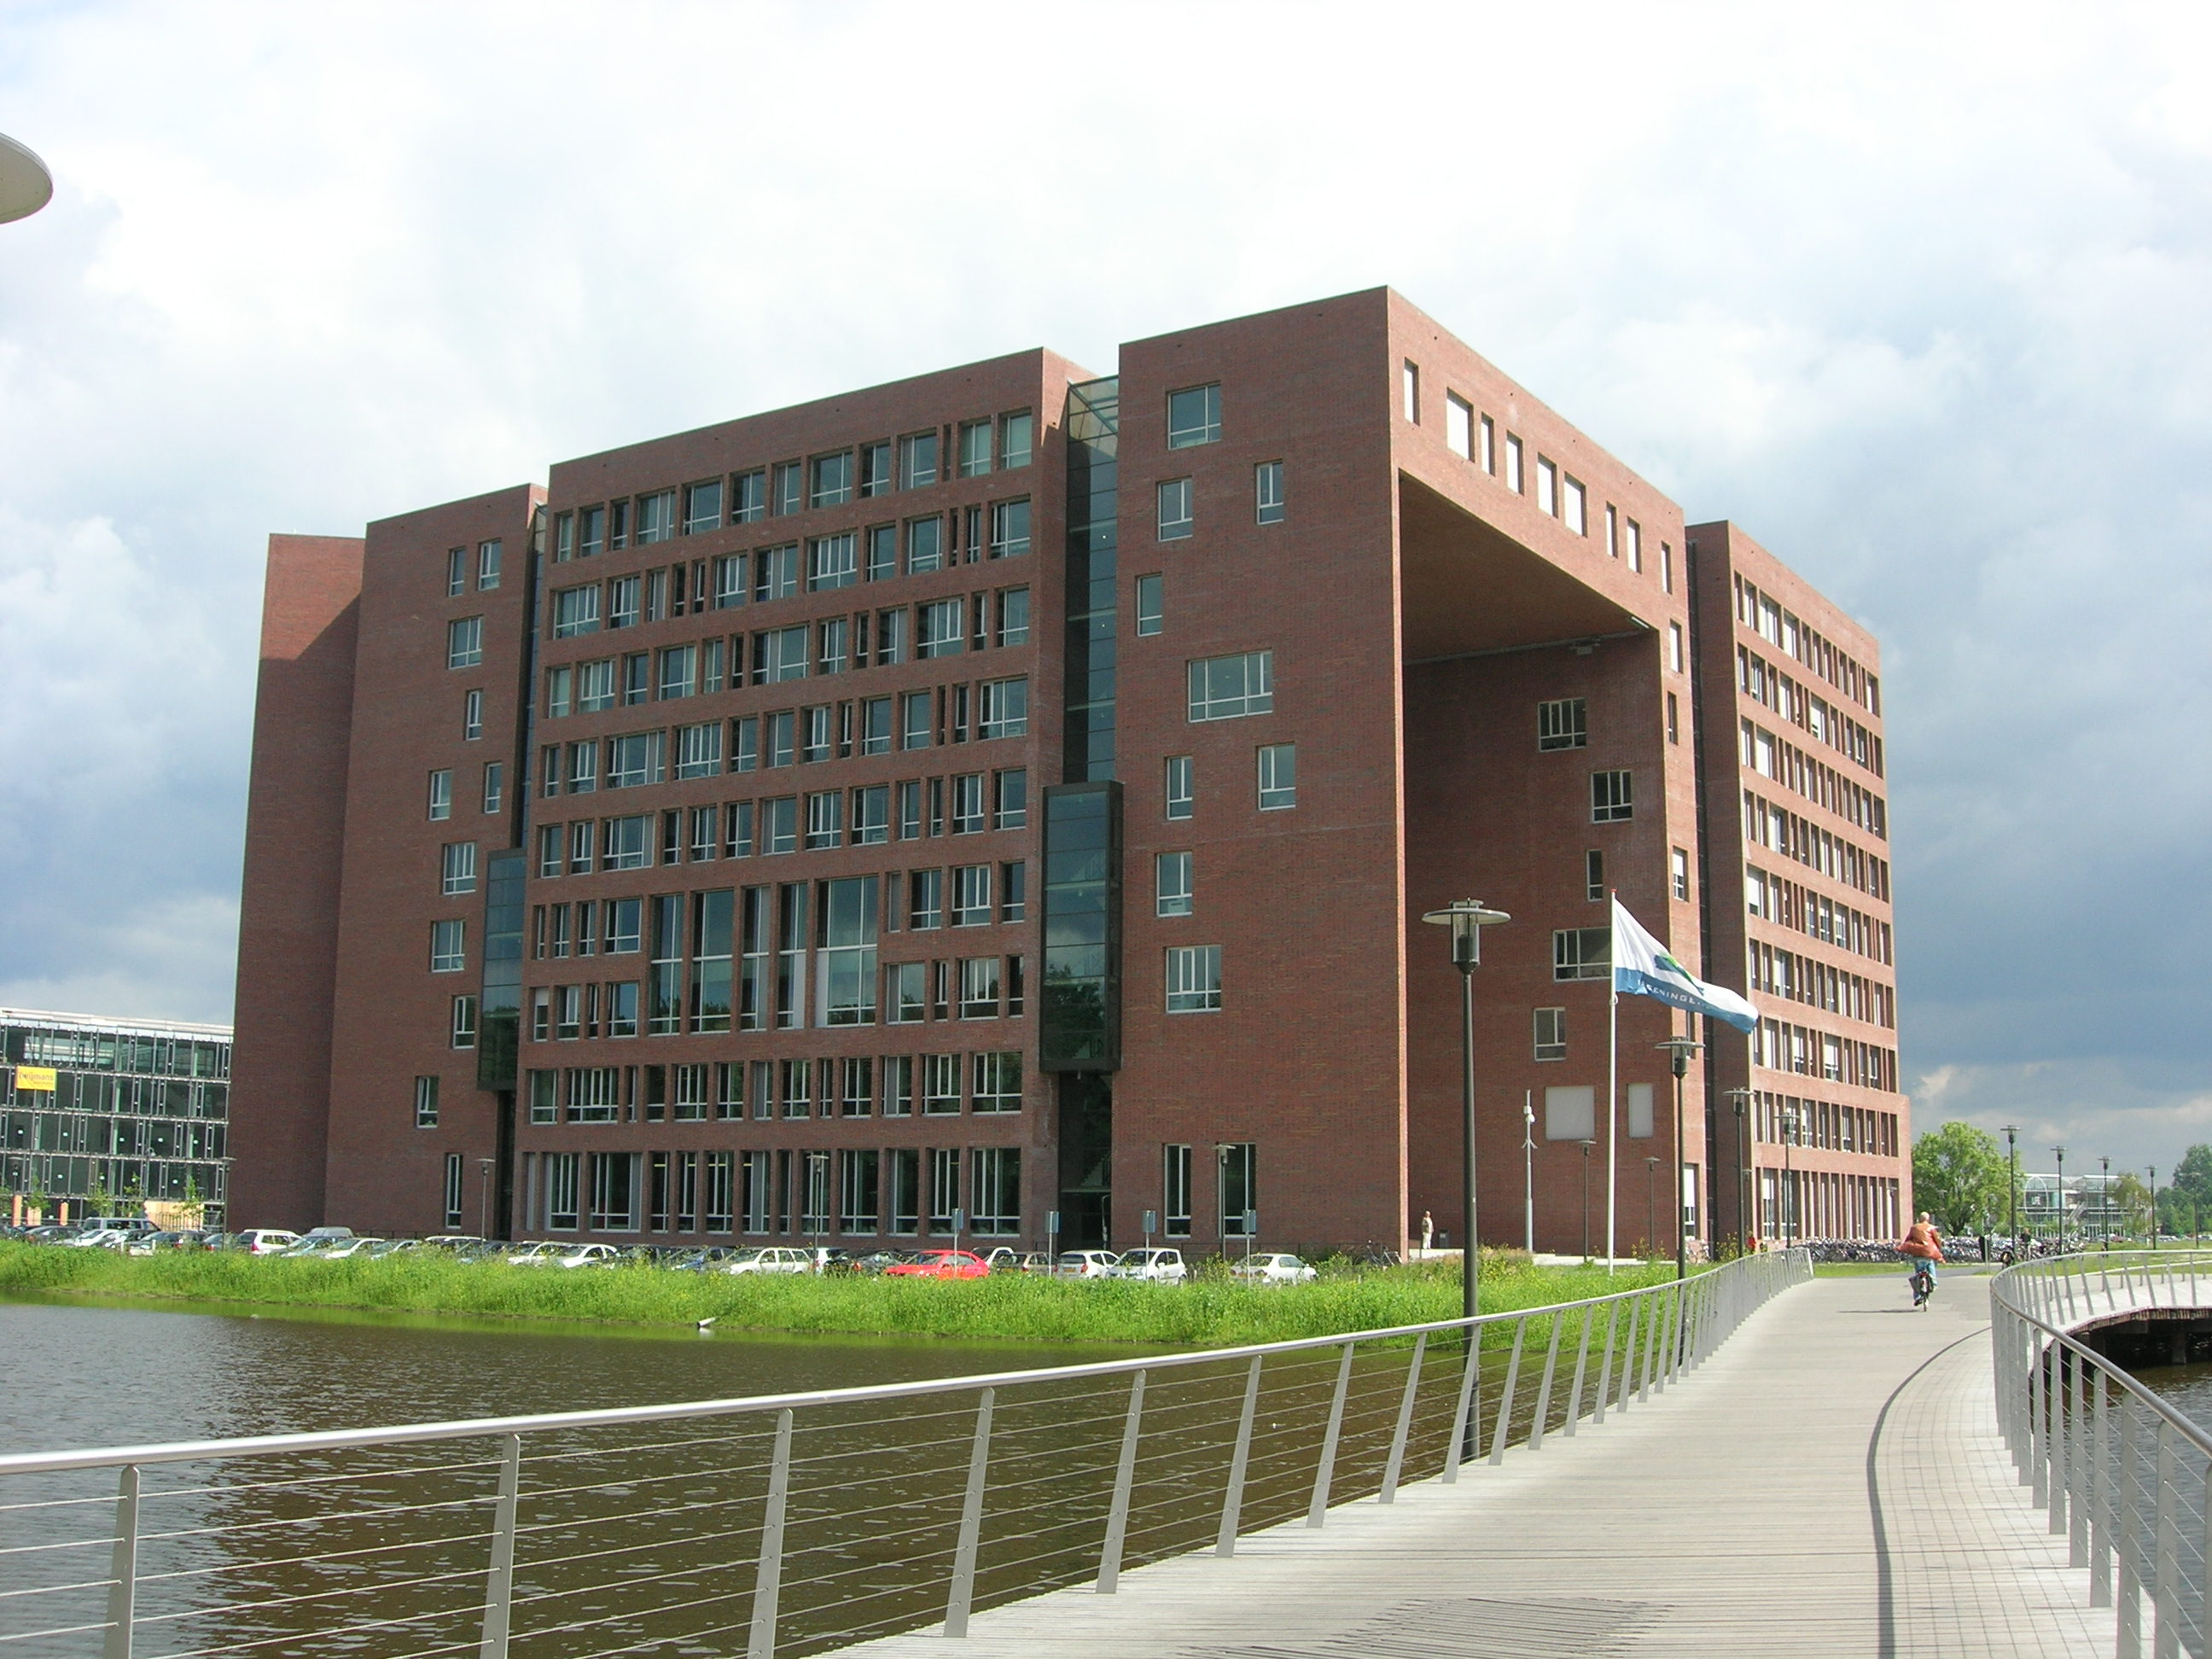
\includegraphics[width=0.75\linewidth]{assets/ch1/WUR_forum_building.jpg}
    \caption{A picture of the Forum building at Wageningen University \& Research.}
    \label{fig:forum_wur_building}
\end{figure}

\lipsum[1-5]      % Generates first 5 paragraphs

\section{Thesis overview}

\lipsum[6]